In questa esperienza si vuole realizzare un misuratore di distanza, utilizzando il sensore di distanza a ultrasuoni. Sono stati utilizzati i seguenti componenti:
\begin{itemize}
    \item Scheda Arduino DUE
    \item Display TFT 3.5" 320x480, \textit{HX8357} Adafruit
    \item Breadboard e cavi
    \item Sensore ultrasonico distanza HC-SR04
\end{itemize}
Il circuito è alimentato mediante porta USB del PC, la quale eroga circa $(\sim 5 V)$
\begin{figure}[H]
    \centering
    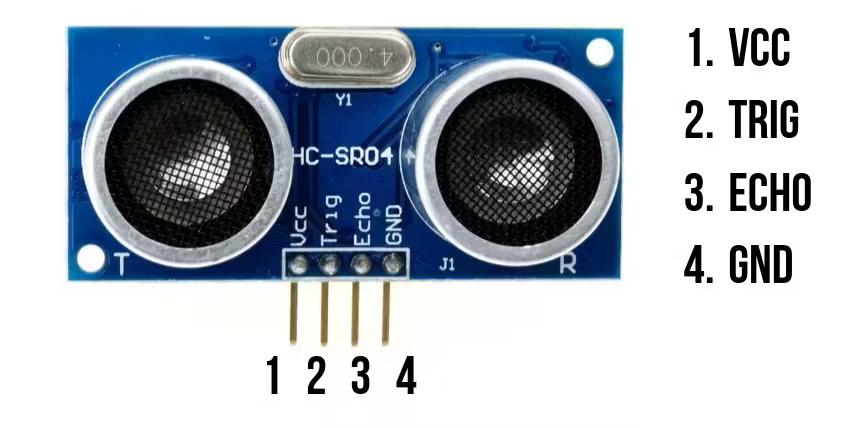
\includegraphics[width=0.5\linewidth]{images/HC-SR04.png}
    \caption{Pinout del sensore HC-SR04}
    \label{fig:HC-SR04}
\end{figure}
\subsection{Codice - interfaccia grafica}
\begin{lstlisting}[frame=single, language=Arduino]
#include <SPI.h>
#include "Adafruit_GFX.h"
#include "Adafruit_HX8357.h"

#define TRIG_PIN 7
#define ECHO_PIN 6

#define TFT_CS 10
#define TFT_DC 9

Adafruit_HX8357 tft = Adafruit_HX8357(TFT_CS, TFT_DC, -1); 

void setup(){
    pinMode(ECHO_PIN, INPUT);
    pinMode(TRIG_PIN, OUTPUT);
    
    // Configurazione del display
    tft.begin();
    tft.setRotation(3);
    tft.fillScreen(HX8357_BLACK);
    tft.setTextColor(HX8357_GREEN);
    tft.setTextSize(6);
    tft.setCursor(60,0);
    tft.println("Distanza");
    tft.setTextColor(HX8357_WHITE);
    tft.setTextSize(10);
}

void loop(){
    String DistTxt = String(distance());
    
    tft.fillRect(0,120,480,320,HX8357_BLACK);
    tft.setCursor(0,150);
    tft.println(DistTxt + " cm");
    
    delay(100);
}
\end{lstlisting}
\subsection{Codice - lettura sensore ultrasonico}
Scrivere cosa fa il codice
\begin{lstlisting}[frame=single, language=Arduino]
long distance(){
    long d = 0;
    long duration = 0;
    
    digitalWrite(TRIG_PIN, LOW);
    delayMicroseconds(2);
    digitalWrite(TRIG_PIN, HIGH);
    delayMicroseconds(2);
    digitalWrite(TRIG_PIN, LOW);
    delayMicroseconds(2);
    
    duration = pulseIn(ECHO_PIN, HIGH);
    d = (duration * 100) / 5830;
    
    delay(25);
    return d;
}
\end{lstlisting}
E' possibile apprezzare il funzionamento del circuito dal video al \href{}{seguente link errato}